\section{Regression Trees}
In a decision tree, there is typically a data set with $N$ features ($X_1, X_2, \cdots, X_N$). Each of the features has a domain, with the domain type being dependent on the type of data the feature contains (categorical or numerical).
The output variable $Y$ will have a domain $D_y$.
\begin{itemize}
    \item Categorical - Classification
    \item Numerical - Regression
\end{itemize}

\subsection{Constructing a Regression Tree}

We have already explored the classification algorithm of decisiont trees and how
entropy, gini and information gain is used to calculate node impurity which is
used to determine the splits. But what do we use when the dependent variable $Y$
is a continious / numerical value? Most litterature use two metrics for 
regression trees are  \textit{Least Squares} and the other 
\textit{Least Absolute deviations}. \cite{loh2011classification} 
In both cases the spread in the nodes is used as a metric for 
\textit{information}, in the same way as entropy. The split that has the least
variance in it's child nodes compared to the parent is the split that contains 
the most information.

\begin{enumerate}
    \item Find a split $(X_i, v)$ that creates two child nodes $D_L$ and $D_R$ from the parent node $D$. The split should maximize the weighted sum of the variances.
    \begin{itemize}
        \item For ordered domains, sort $X_i$ and consider a split between each pair of adjacent values.
        \item For categorical $X_i$ find the best split based on subsets (Breiman's algorithm).
    \end{itemize}
\end{enumerate}

\begin{equation}
    \text{Weighted Variance} = \abs{D}*Var(D) - \left(\abs{D_L}*Var(D_L) + \abs{D_R}*Var(D_R)\right)
\end{equation}

\begin{equation}
    \text{Var}(D) = \frac{1}{n}\sum_{i=1}^{\abs{D}}(y_i-\overline{y})^2
\end{equation}

\subsubsection{Stopping a Tree}
\begin{itemize}
    \item When the leaf is pure, i.e. $Var(D) < \epsilon$
    \item When the number of instances in the leaf $(\abs{D})$ is too small.
\end{itemize}

\subsubsection{Predictor}
\begin{itemize}
    \item Regression - Average value of $y_i$ of the instances in the leaf.
    \item Classification - Choose the most common $y_i$ in the leaf.
\end{itemize}

\section{Ensemble Methods}
In addition to using pruning to construct more generalised trees. Two other
methods exist to generalise models. These are ensemble and resample methods.
Ensemble methods construct a set of classifiers from a given training data.
The classification is done by predicting class values from previously unseen 
records by aggregating predictions made by multiple classifiers.

\bigskip
The general idea of ensemble methods is to have the original training data and then:
\begin{enumerate}
    \item Create multiple data sets from the training data (resampling).
    \item Build multiple classifiers corresponding to the data sets.
    \item Combine the predictions of the classifiers.
\end{enumerate}

Ensemble methods work the sum of the error rate of multiple independent classifiers are lower than the error rate itself.
The following equation calculates the probability that the ensemble classifier makes a wrong prediction, having $\epsilon$ as the error rate.

\begin{equation}
    \sum_{i=N/2(+1)}^N \genfrac(){0pt}{2}{N}{i} \epsilon^i(1-\epsilon)^{N-i}
\end{equation}

\section{Manipulating the Training set}
\subsubsection{Bagging}
Bagging is sampling with replacement (bootstrapping).

\begin{enumerate}
    \item Let $k$ be the number of bootstrap samples.
    \item \texttt{for $i$ in range($k$):}
    \begin{enumerate}
        \item Create a bootstrap sample of size $N$, $D_i$.
        \item Train a base classifier $C_i$ on the bootstrap sample $D_i$.
    \end{enumerate}
    $C^{*}(x) = argmax\left(\sum_i \delta\left(C_i(x)=y\right)\right)$
\end{enumerate}

$\delta = 1$ if the argument is true and $0$ otherwise (the majority class is chosen).

Bagging can also increase the complexity of simple classifiers such as decision stumps.

\newpage
\subsubsection{Boosting}
Boosting is an iterative procedure to adaptively change the distribution of training data by focusing more on previously misclassified records.
Initially, all $N$ records are assigned equal weights.

Unlike bagging, the weights of the records may change at the end of each boosting round.

\begin{itemize}
    \item Records that are wrongly classified will have their weights increased.
    \item Records that are classified correctly will have their weights decreased.
\end{itemize}

One way of boosting is to use the AdaBoost algorithm:

\begin{figure}[H]
    \centering
    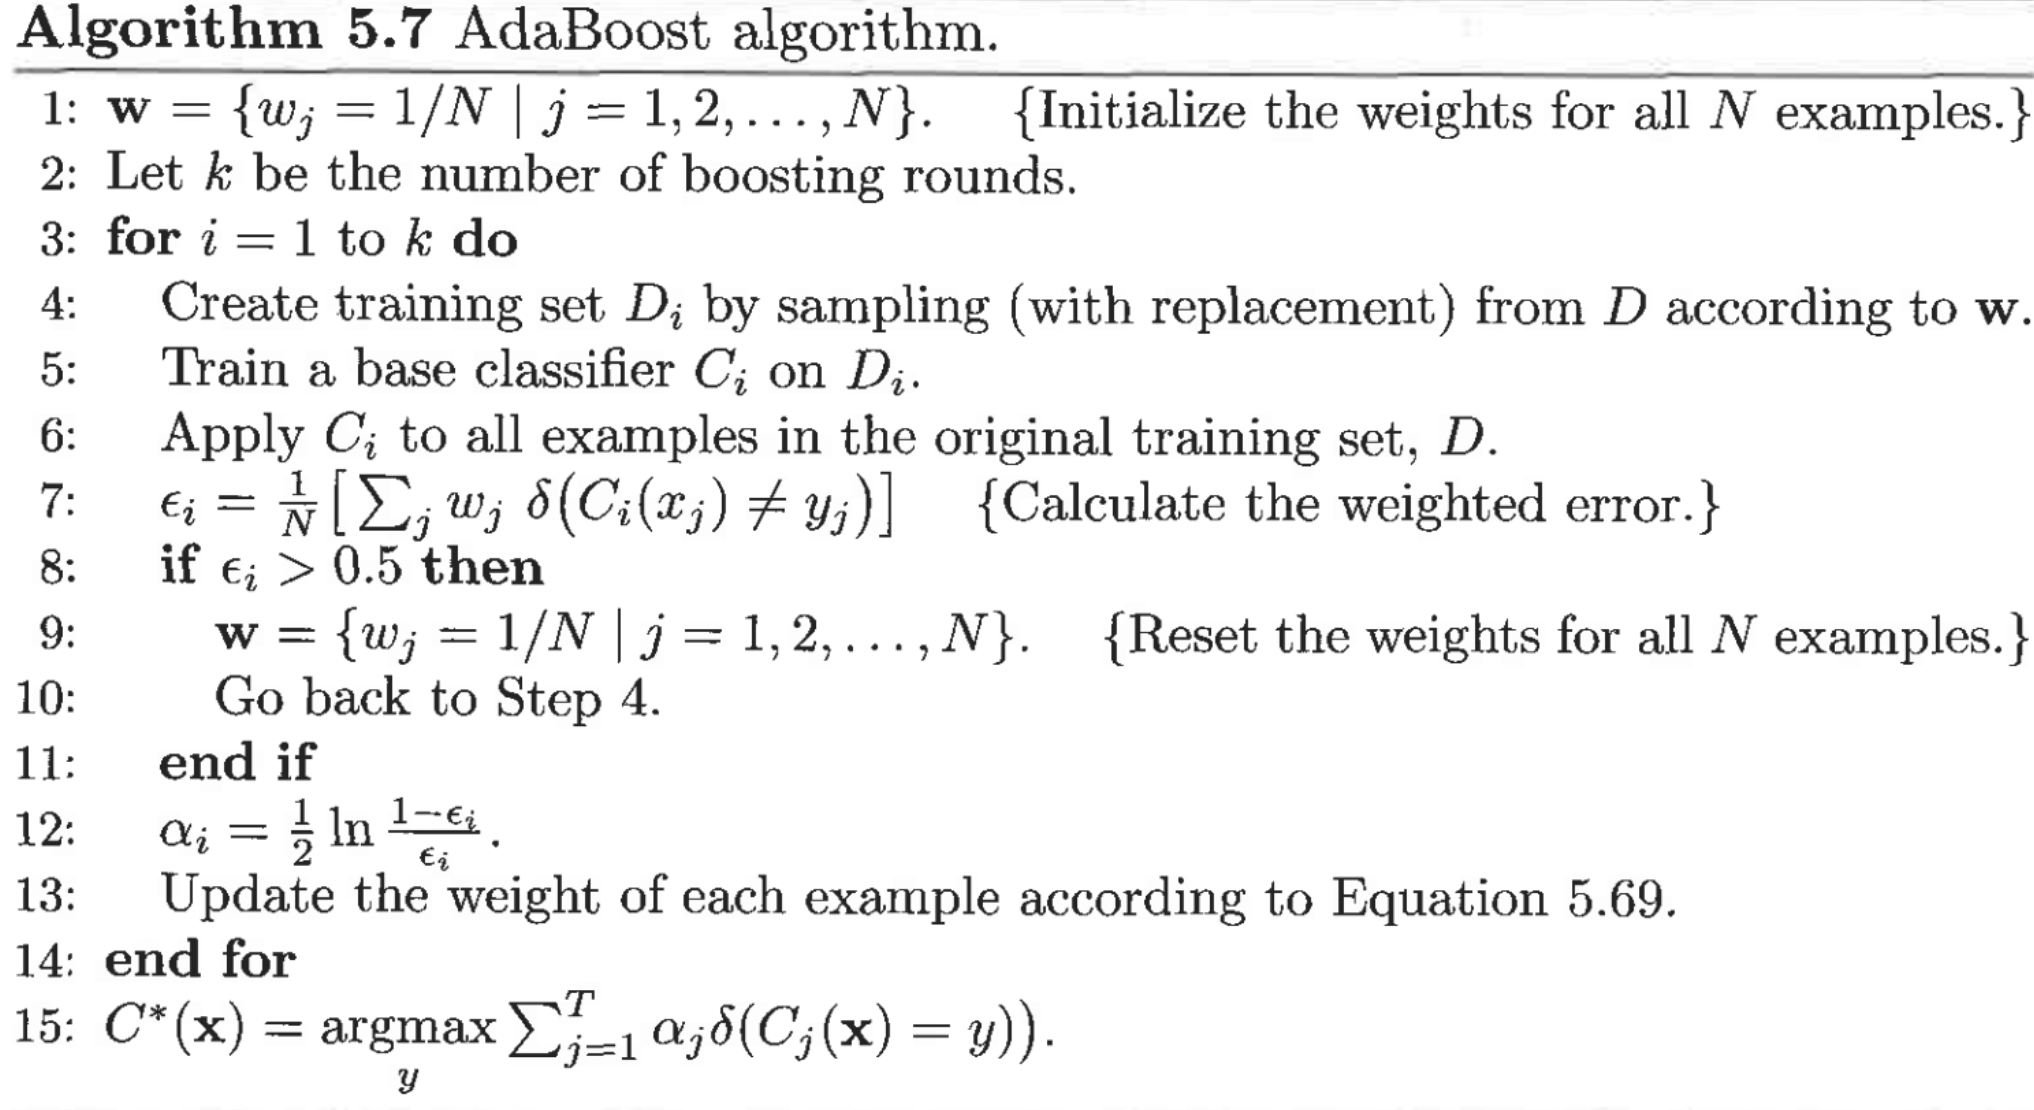
\includegraphics[scale=0.3]{figures/adaboost.png}
    \caption{AdaBoost Algorithm}
\end{figure}

\newpage
\section{Manipulating the Features}
\subsubsection{Random Forest}
A random forest is a class of ensemble methods specifically designed for decision tree classifiers.
It combines the predictions made by multiple decision trees where each tree is generated based on the values of an independent sample set.
The samples are generated from a fixed probability distribution.

\bigskip
As in bagging, we build decision trees on bootstrapped training samples.
Each time a split in a tree is considered, a random sample of $F$ features is chosen as split candidates from the full set of $m$ features.

(If $F=m$, we have bagging)

\bigskip
A random forest algorithm can look like this:
\begin{itemize}
    \item \texttt{for $i$ in range($B$):}
\end{itemize}
\begin{enumerate}
    \item Draw a bootstrap sample $D^{*}$ of size $N$ from the training data.
    \begin{enumerate}
        \item Grow a random forest tree to the bootstrapped data.
        \begin{enumerate}
            \item Select $\bm{F}$ features at random from the $m$ variables.
            \item Pick the best variable/split point among the $\bm{F}$s.
            \item Split the node into two child nodes.
        \end{enumerate}
    \end{enumerate}
\end{enumerate}
\begin{itemize}
    \item Output the ensemble of trees.
\end{itemize}

Prediction at a new point $x$ can be done:
\begin{itemize}
    \item For regression - Average of the results.
    \item For classification - Majority vote.
\end{itemize}

\subsubsection{Random Forest Recommendations}
\begin{itemize}
    \item For classification, the default value for $F$ is $\sqrt{m}$ and the minimum node size is one.
    \item For regression, the default value for $F$ is $\frac{m}{3}$ and the minimum node size is five.
\end{itemize}
